\subsubsection{Dijkstra}
The Dijkstra controller lets user perform Dijkstra's Shortest Path First algorithm on a given graph.
\begin{figure}[H]
    \centering
    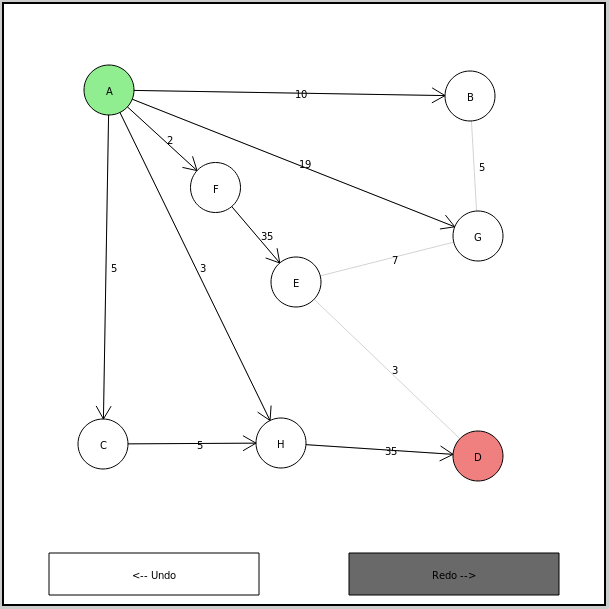
\includegraphics[width=0.7\linewidth]{/graphdrawer/dijkstraui}
    \caption{Dijkstra - user interface}
    \label{fig:graphdrawerDijkstraUserInterface}
\end{figure}
If the Dijkstra controller is not given a configuration object, then it will only display a white screen without allowing any user interaction. This happens becuase this controller is made for finding the shortest path, or for showing how the algorithm finds the shortest path. It can not be used to create a graph. The following properties can be determined by the configuration object:
\begin{enumerate}
    \item \code{steps}, should be an array of the steps the algorithm uses to find the shortest path. This can be undefined, if the intention is for the student to use the algorithm to find the path. If \code{steps} is defined, then the \code{graph} configuration is not needed.
    \item \code{startColor}, the fill color used for the start node.
    \item \code{endColor}, the fill color used for the end node.
    \item \code{edgeColor}, is the color used for lines which show the path between nodes.
    \item \code{graph}, contains information about the graph which the student should use the algorithm on. The following list is all of the possible properties on the \code{graph} object.
    \begin{itemize}
        \item \code{graph}, contains the graph.
        \item \code{from}, should be the starting node.
        \item \code{to}, should be the end node.
        \item \code{nodes}, should be an array of node objects which the graph consists of.
    \end{itemize}
\end{enumerate}
The Dijkstra controller uses the steps array to store operations. There are three step types:
\begin{enumerate}
    \item \code{"Initial"}, is used to store information about the graph. It has the same properties as the \code{graph} configuration object.
    \item \code{"Distance"}, is used to show that the algorithm is checking the cost between to nodes. 
\end{enumerate}